\documentclass[conference]{../../LaTex_Template/IEEEtran}
\IEEEoverridecommandlockouts
\usepackage{cite}
\usepackage{amsmath,amssymb,amsfonts}
\usepackage{graphicx}
\usepackage{textcomp}
\usepackage{float}
\graphicspath{{../../../results/figures/}{../figures/}}

\begin{document}

\title{Dynamic Pricing with Demand Learning and Reference Effects: Replication and Robust Calibration}

\author{
\IEEEauthorblockN{Jingwen Luo}
\IEEEauthorblockA{Student ID: 72542176\\
SDSC8008 Data-driven Operations Research}
}

\maketitle

\begin{abstract}
This report studies den Boer and Keskin's dynamic pricing model with demand learning and reference effects. The project has three goals. The first is to explain why reference-price effects make dynamic pricing different from a standard learning-and-earning problem. The second is to reproduce the main numerical evidence in the paper. The third is to add a small operations-research extension that calibrates the slow-moving policy under uncertainty about reference-price memory and loss-side reference effects. For rigor, the converted numerical results from the published study are called the Published Study Benchmark (PSB), and the new project simulations are called the Independent Replication Experiment (IRE). The report uses PSB and IRE hereafter. The IRE reproduces the paper's main lesson: deterministic testing works well without reference effects but suffers high regret when reference effects are present, whereas slow-moving pricing remains stable. The extension, called Reference-Aware Robust Calibration (RARC), shows that a smaller initial perturbation and slower perturbation decay can improve worst-case regret over the tested uncertainty set.
\end{abstract}

\section{Background, Motivation, and Core Idea}
Dynamic pricing is a central topic in data-driven operations research. A seller repeatedly chooses prices, observes demand, updates its estimate of the demand curve, and tries to maximize long-run revenue. Even without behavioral effects, the problem has a basic learning-and-earning tension. A seller needs price variation to estimate demand, but price experiments may reduce current revenue. A large literature studies this tradeoff under unknown demand parameters and current-price dependent demand \cite{broderRusmevichientong2012,keskinZeevi2014}.

The paper studied in this project adds a behavioral state variable: the reference price. Consumers often evaluate the current price relative to a remembered or expected price. A price below the reference point may look like a gain, while a price above it may look like a loss. This idea is closely related to reference-dependent preferences and loss aversion \cite{tverskyKahneman1991}. In pricing applications, reference effects help explain why temporary discounts, repeated promotions, and abrupt price increases may affect future willingness to buy \cite{popescuWu2007}.

The operational difficulty is that the reference price is endogenous. It is formed by past prices and then affects future demand. Therefore, a price experiment has two effects at the same time. It creates information for demand estimation, and it changes the state in which future demand will be observed. This is the key reason why the problem is not just a standard regression problem with online data. If the seller uses a policy designed for a no-reference model, the policy may confuse reference-state movements with price-slope or demand-intercept effects. The estimated optimal price can then converge to the wrong level.

The core idea of den Boer and Keskin's paper is to design learning and state control jointly. Price variation must be informative, but it must not move the reference state too aggressively. The slow-moving policy implements this idea through increasingly long episodes and shrinking two-sided perturbations around the estimated optimal price. Within an episode, price changes are gradual enough for the reference price to move toward the posted prices. This makes the observed demand closer to the environment assumed by the estimator.

This report focuses on the numerical and operational meaning of that idea. The replication compares deterministic testing and slow-moving pricing. Deterministic testing is natural in a no-reference model: it periodically posts two test prices and otherwise posts the estimated optimum. Slow-moving pricing deliberately controls the pace of price changes. The central question is whether the observed regret and price-estimate paths support the paper's claim that, with reference effects, policy structure matters more than simply collecting more demand data.

Figure~\ref{fig:referencefeedback} summarizes the feedback mechanism. The same posted price enters current demand, current revenue, future reference-price updating, and the next learning step. This is the reason exploration must be evaluated as both data collection and state intervention.

\begin{figure*}[!t]
  \centering
  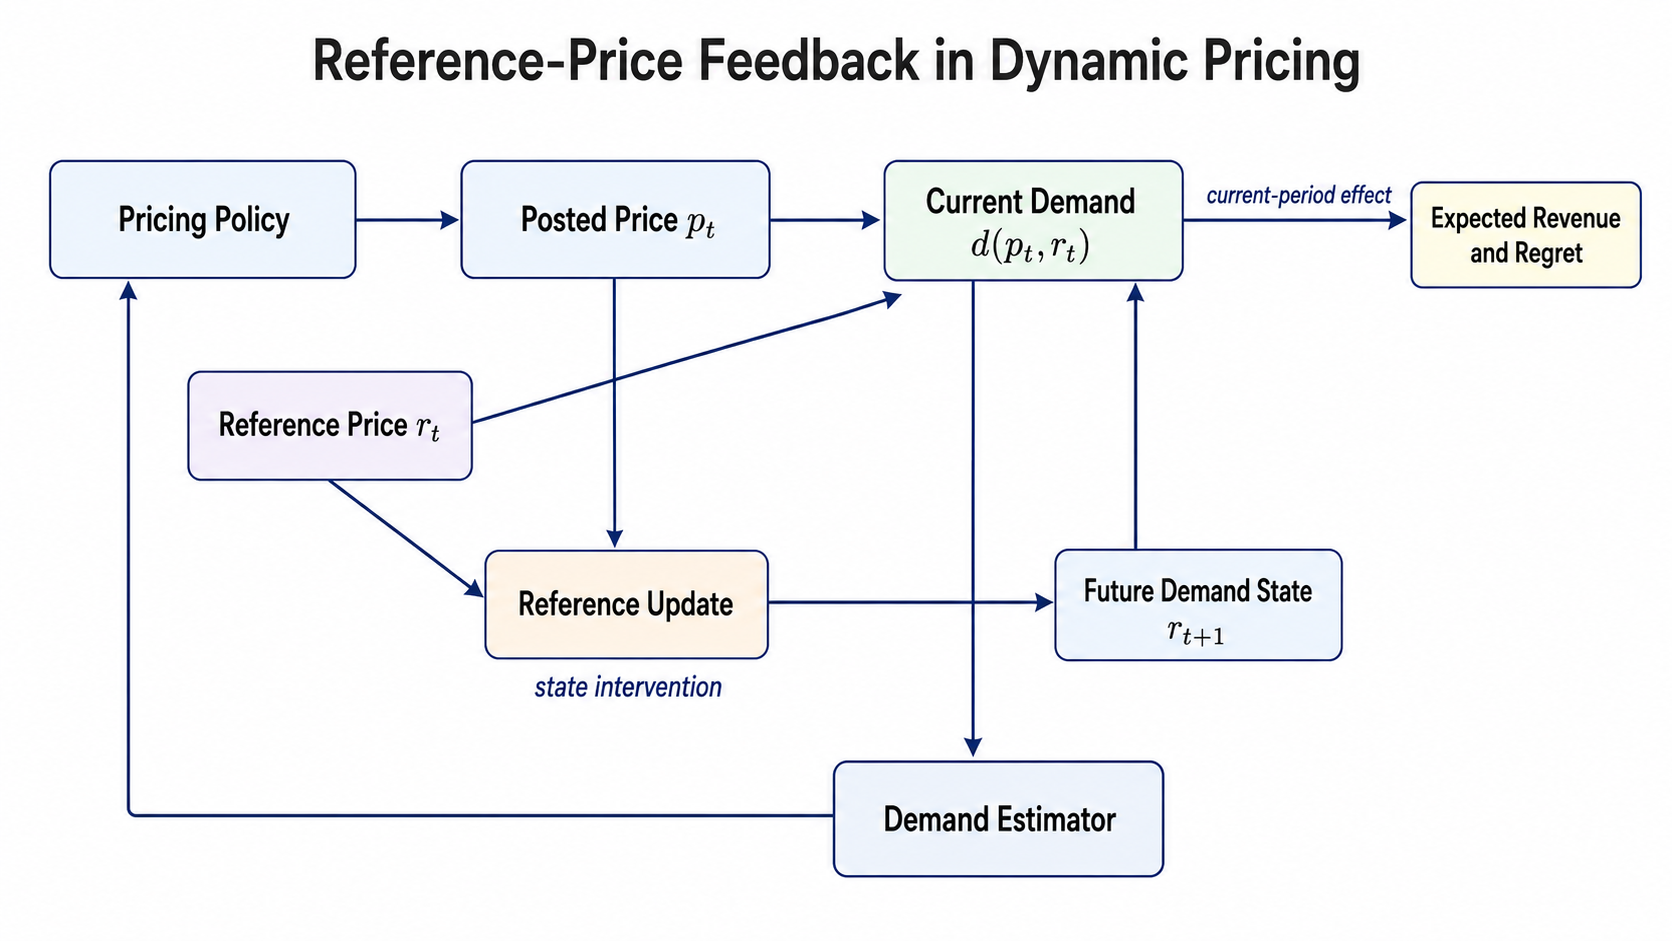
\includegraphics[width=0.92\textwidth]{reference_feedback.png}
  \caption{Reference-price feedback mechanism. A price action affects current demand and also changes the reference state used in future demand observations.}
  \label{fig:referencefeedback}
\end{figure*}

\section{Model, Theory, and Application}
\subsection{Demand Model}
The replicated demand model is
\begin{equation}
d_t = \alpha - \beta p_t + \eta^+(r_t-p_t)^+ - \eta^-(p_t-r_t)^+ + \epsilon_t,
\label{eq:demand}
\end{equation}
where $p_t$ is the posted price, $r_t$ is the reference price, and $\epsilon_t$ is a zero-mean demand shock. The IRE uses the positive price-sensitivity notation $\beta>0$, so the direct price effect is $-\beta p_t$. The term $\eta^+(r_t-p_t)^+$ captures the gain-side effect when price is below the reference price. The term $-\eta^-(p_t-r_t)^+$ captures the loss-side effect when price is above the reference price. The reference-effect environment used in the main experiments has $\eta^+=0.1$ and $\eta^-=0.3$, so losses matter more than gains.

The time-varying reference price follows exponential smoothing:
\begin{equation}
r_{t+1} = \zeta r_t + (1-\zeta)p_t,\quad \zeta \in [0,1).
\label{eq:reference}
\end{equation}
When $\zeta$ is small, the reference price reacts quickly to the current price. When $\zeta$ is larger, the reference price has longer memory. The main replication uses $\zeta=0.1$. The robust-calibration extension varies $\zeta$ because memory length is one of the most important uncertainties in applied pricing.

For a given reference price, expected single-period revenue is
\begin{equation}
R(p,r,\theta)=p\left[\alpha-\beta p+\eta^+(r-p)^+-\eta^-(p-r)^+\right],
\end{equation}
where $\theta=(\alpha,\beta,\eta^+,\eta^-)$. If reference effects vanish or are ignored, the static optimal price is $\alpha/(2\beta)$, clipped to the feasible price interval. With $\alpha=1.1$ and $\beta=0.5$, the benchmark price is $p^\star=1.1$.

\subsection{Regret and Theoretical Logic}
The paper evaluates a policy $\pi$ using cumulative regret:
\begin{equation}
\Delta_\pi(T,\rho,\theta)=\Pi^\star(T,\rho,\theta)
-\mathbb{E}_\pi\left[\sum_{t=1}^T R(p_t,r_t,\theta)\right].
\end{equation}
The benchmark is a full-information decision maker that knows the demand parameters and the reference-price process. The exact dynamic benchmark can be hard to characterize, but the paper shows that the fixed price $p^\star=\alpha/(2\beta)$ is a powerful comparison point in the loss-averse time-varying reference-price setting. If the seller posts a fixed price, the reference price converges geometrically to it, so the cumulative loss caused by reference-price mismatch can be controlled.

The theoretical mechanism can be summarized in three steps. First, a stable price path keeps the reference state from drifting in a harmful way. Second, if prices are held nearly constant over longer episodes, the state contamination in demand observations becomes smaller. Third, shrinking perturbations still provide enough price variation for learning. The slow-moving policy balances these three forces and obtains $O(\sqrt{T})$ regret, matching the basic lower-bound order for unknown-demand pricing. Deterministic testing fails in the reference-effect setting because it treats forced price variation as information collection only, not as state intervention.

\subsection{Application Interpretation}
The model is relevant to repeated retail pricing, subscription renewal pricing, online platform experimentation, and promotion calendars. In these settings, customers may learn from posted prices and form expectations about what a fair or normal price should be. A firm that discounts too frequently may lower the reference price. A firm that raises prices abruptly may trigger perceived losses. The paper's managerial message is not that price experimentation should stop. Rather, experimentation must account for how current tests reshape future customer expectations.

From an operations-research perspective, slow-moving pricing is a disciplined experimental design. It uses local and gradual price perturbations, not aggressive random exploration. This makes the policy interpretable: one part of the price path is used for estimation, while the episode structure controls the latent state. This separation is also useful for implementation, because it can be explained to managers as a controlled testing protocol rather than a black-box algorithm.

\section{IRE Design and Terminology}
\subsection{PSB and IRE}
The numerical comparison uses two sources. Published Study Benchmark (PSB) refers to the released numerical outputs from the published study after conversion into structured arrays and CSV files. Independent Replication Experiment (IRE) refers to the new simulation outputs generated by this project from the stated demand and reference-price equations. The PSB is used only for comparison and visualization. The IRE generates fresh paths with deterministic random seeds.

This distinction matters for interpretation. The IRE is not expected to match each PSB path point by point because the random streams are not matched. The relevant comparison is whether the policy ranking, curve shape, final magnitude, and mechanism-level interpretation agree. This is also why the reports and figures show three views: PSB alone, IRE alone, and an overlay in a shared coordinate system.

\subsection{Pipeline and Parameters}
The pipeline has three stages. First, the released study outputs are converted to `.npz' and CSV files under `data/processed/'. Second, the IRE runs deterministic-testing and slow-moving simulations under the same main parameter settings. Third, the plotting module creates Figure 2--5 comparisons and a summary CSV table.

Figure~\ref{fig:pipelineworkflow} shows the implemented replication pipeline. The PSB stream provides benchmark curves after conversion, while the IRE stream generates fresh simulation curves from the Python model modules. The two streams meet only at the visualization and summary stage.

\begin{figure*}[!t]
  \centering
  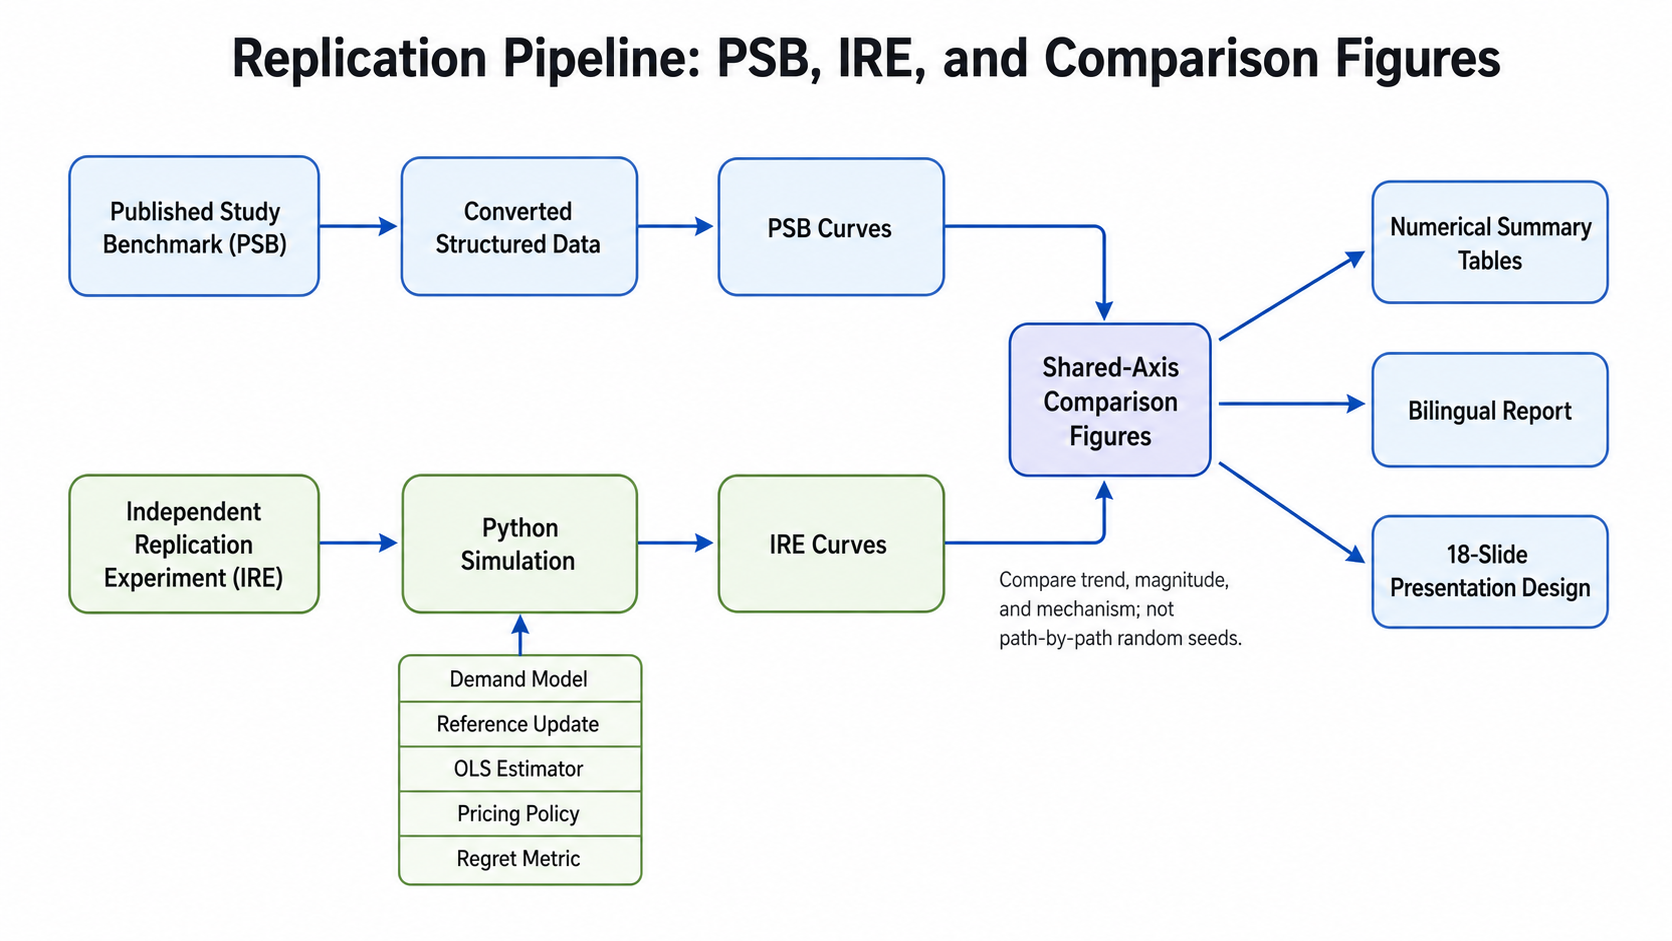
\includegraphics[width=0.92\textwidth]{replication_pipeline.png}
  \caption{Replication pipeline. PSB and IRE outputs are kept separate until shared-axis comparison figures and numerical summaries are produced.}
  \label{fig:pipelineworkflow}
\end{figure*}

The main parameters are $\alpha=1.1$, $\beta=0.5$, $\sigma=0.1$, $\zeta=0.1$, horizon $T=10000$, ten simulation paths, and price interval $[0.5,1.5]$. Two demand environments are used. The no-reference environment sets $\eta^+=\eta^-=0$. The reference-effect environment sets $\eta^+=0.1$ and $\eta^-=0.3$. Regret is computed using expected revenue. Realized demand is used only to update the estimators, so random shocks are not mixed into the theoretical revenue comparison.

\subsection{Implemented Policies}
Deterministic testing uses two fixed exploration prices at one third and two thirds of the feasible interval. With the default interval, the test prices are approximately $0.8333$ and $1.1667$. Outside forced testing periods, the policy estimates a linear demand model and posts
\begin{equation}
\hat p_t^\star = \frac{\hat\alpha_t}{2\hat\beta_t},
\end{equation}
clipped to the feasible interval. This policy is statistically natural under a no-reference model, but it ignores the reference state.

Slow-moving pricing is episode based. In episode $i$, the policy prices below and above the current estimated optimum using a perturbation $\delta_i$. The half-episode length grows as $n_i=2^i$, and the perturbation shrinks as $\delta_i=c_0 2^{-i/4}$ in the main replication. At the end of each episode, the policy updates the estimated demand parameters and the estimated optimal price. Longer episodes help the reference price approach the current price level, while two-sided perturbations preserve local price variation.

\section{Replication Results}
\subsection{Final-Period Summary}
Table~\ref{tab:comparison} summarizes the final-period comparison. The IRE reproduces the main ranking in the PSB. Deterministic testing has low regret without reference effects, but its regret becomes large when reference effects are present. Slow-moving pricing keeps regret low in both environments.

\begin{table*}[t]
\centering
\caption{Final-period comparison between PSB and IRE results.}
\label{tab:comparison}
\begin{tabular}{llllrrr}
\hline
Figure & Policy & Scenario & Metric & PSB & IRE & Relative diff.\\
\hline
2 & Deterministic testing & No reference & Final mean regret & 12.18 & 9.67 & -20.63\%\\
2 & Deterministic testing & Reference effect & Final mean regret & 328.79 & 299.51 & -8.90\%\\
3 & Deterministic testing & No reference & Final mean price estimate & 1.095 & 1.090 & -0.45\%\\
3 & Deterministic testing & Reference effect & Final mean price estimate & 0.850 & 0.860 & 1.24\%\\
4 & Slow-moving & Reference effect & Final mean reference price & 1.097 & 1.076 & -1.90\%\\
4 & Slow-moving & Reference effect & Final mean price estimate & 1.109 & 1.088 & -1.88\%\\
5 & Slow-moving & No reference & Final mean regret & 7.61 & 11.86 & 55.88\%\\
5 & Slow-moving & Reference effect & Final mean regret & 10.40 & 12.33 & 18.59\%\\
\hline
\end{tabular}
\end{table*}

\subsection{Deterministic Testing}
Figure~\ref{fig:figure2} shows the regret comparison for deterministic testing. In the no-reference environment, both PSB and IRE curves remain low. The final mean regret is $12.18$ for PSB and $9.67$ for IRE, which is small relative to the horizon of $10000$. This confirms that deterministic testing can learn effectively when the model it estimates matches the data-generating process.

The reference-effect environment is different. Final regret rises to $328.79$ for PSB and $299.51$ for IRE. The overlay panels show the same qualitative shape: regret accumulates much faster once reference effects are present. The policy is still collecting data, but the data are contaminated by a state variable that the policy does not model.

\begin{figure*}[t]
  \centering
  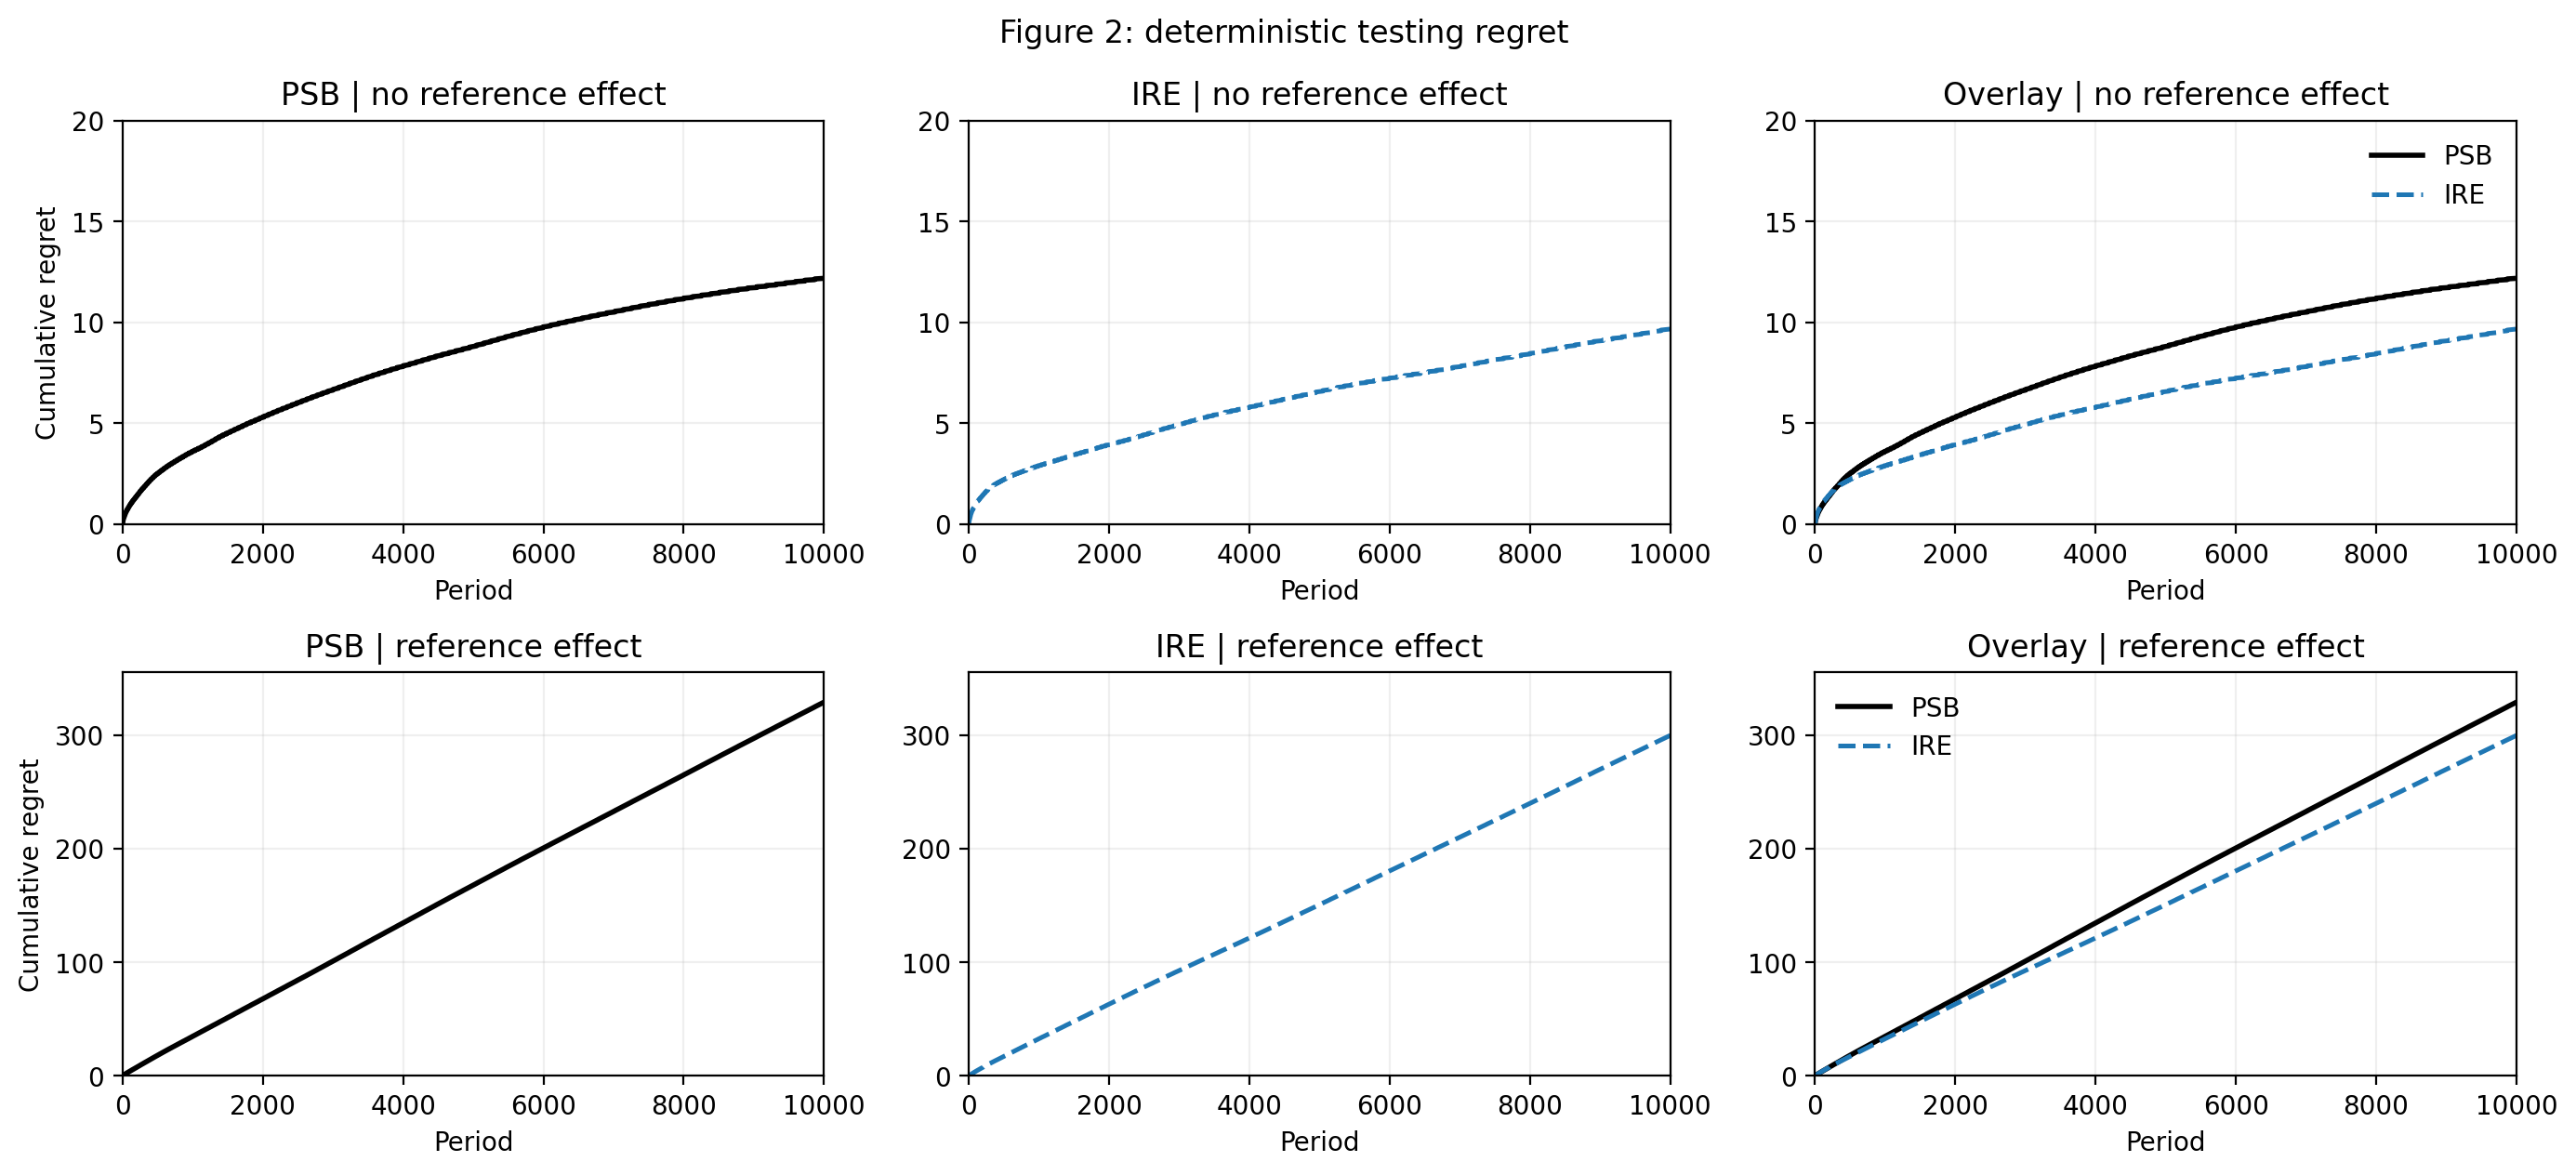
\includegraphics[width=0.96\textwidth]{figure2_comparison.png}
  \caption{Figure 2 comparison. Each row is an environment; columns show PSB, IRE, and overlay views for deterministic-testing regret.}
  \label{fig:figure2}
\end{figure*}

Figure~\ref{fig:figure3} explains the failure mechanism. Without reference effects, the estimated price converges near $p^\star=1.1$. With reference effects, the final mean price estimate is around $0.85$--$0.86$, far below the benchmark. This is not a numerical failure of least squares. It is model misspecification. Demand depends on both price and the reference state, while the regression treats price as the main explanatory variable. Because the reference state is generated by past prices, its effect is partially absorbed into the estimated intercept and slope.

\begin{figure*}[t]
  \centering
  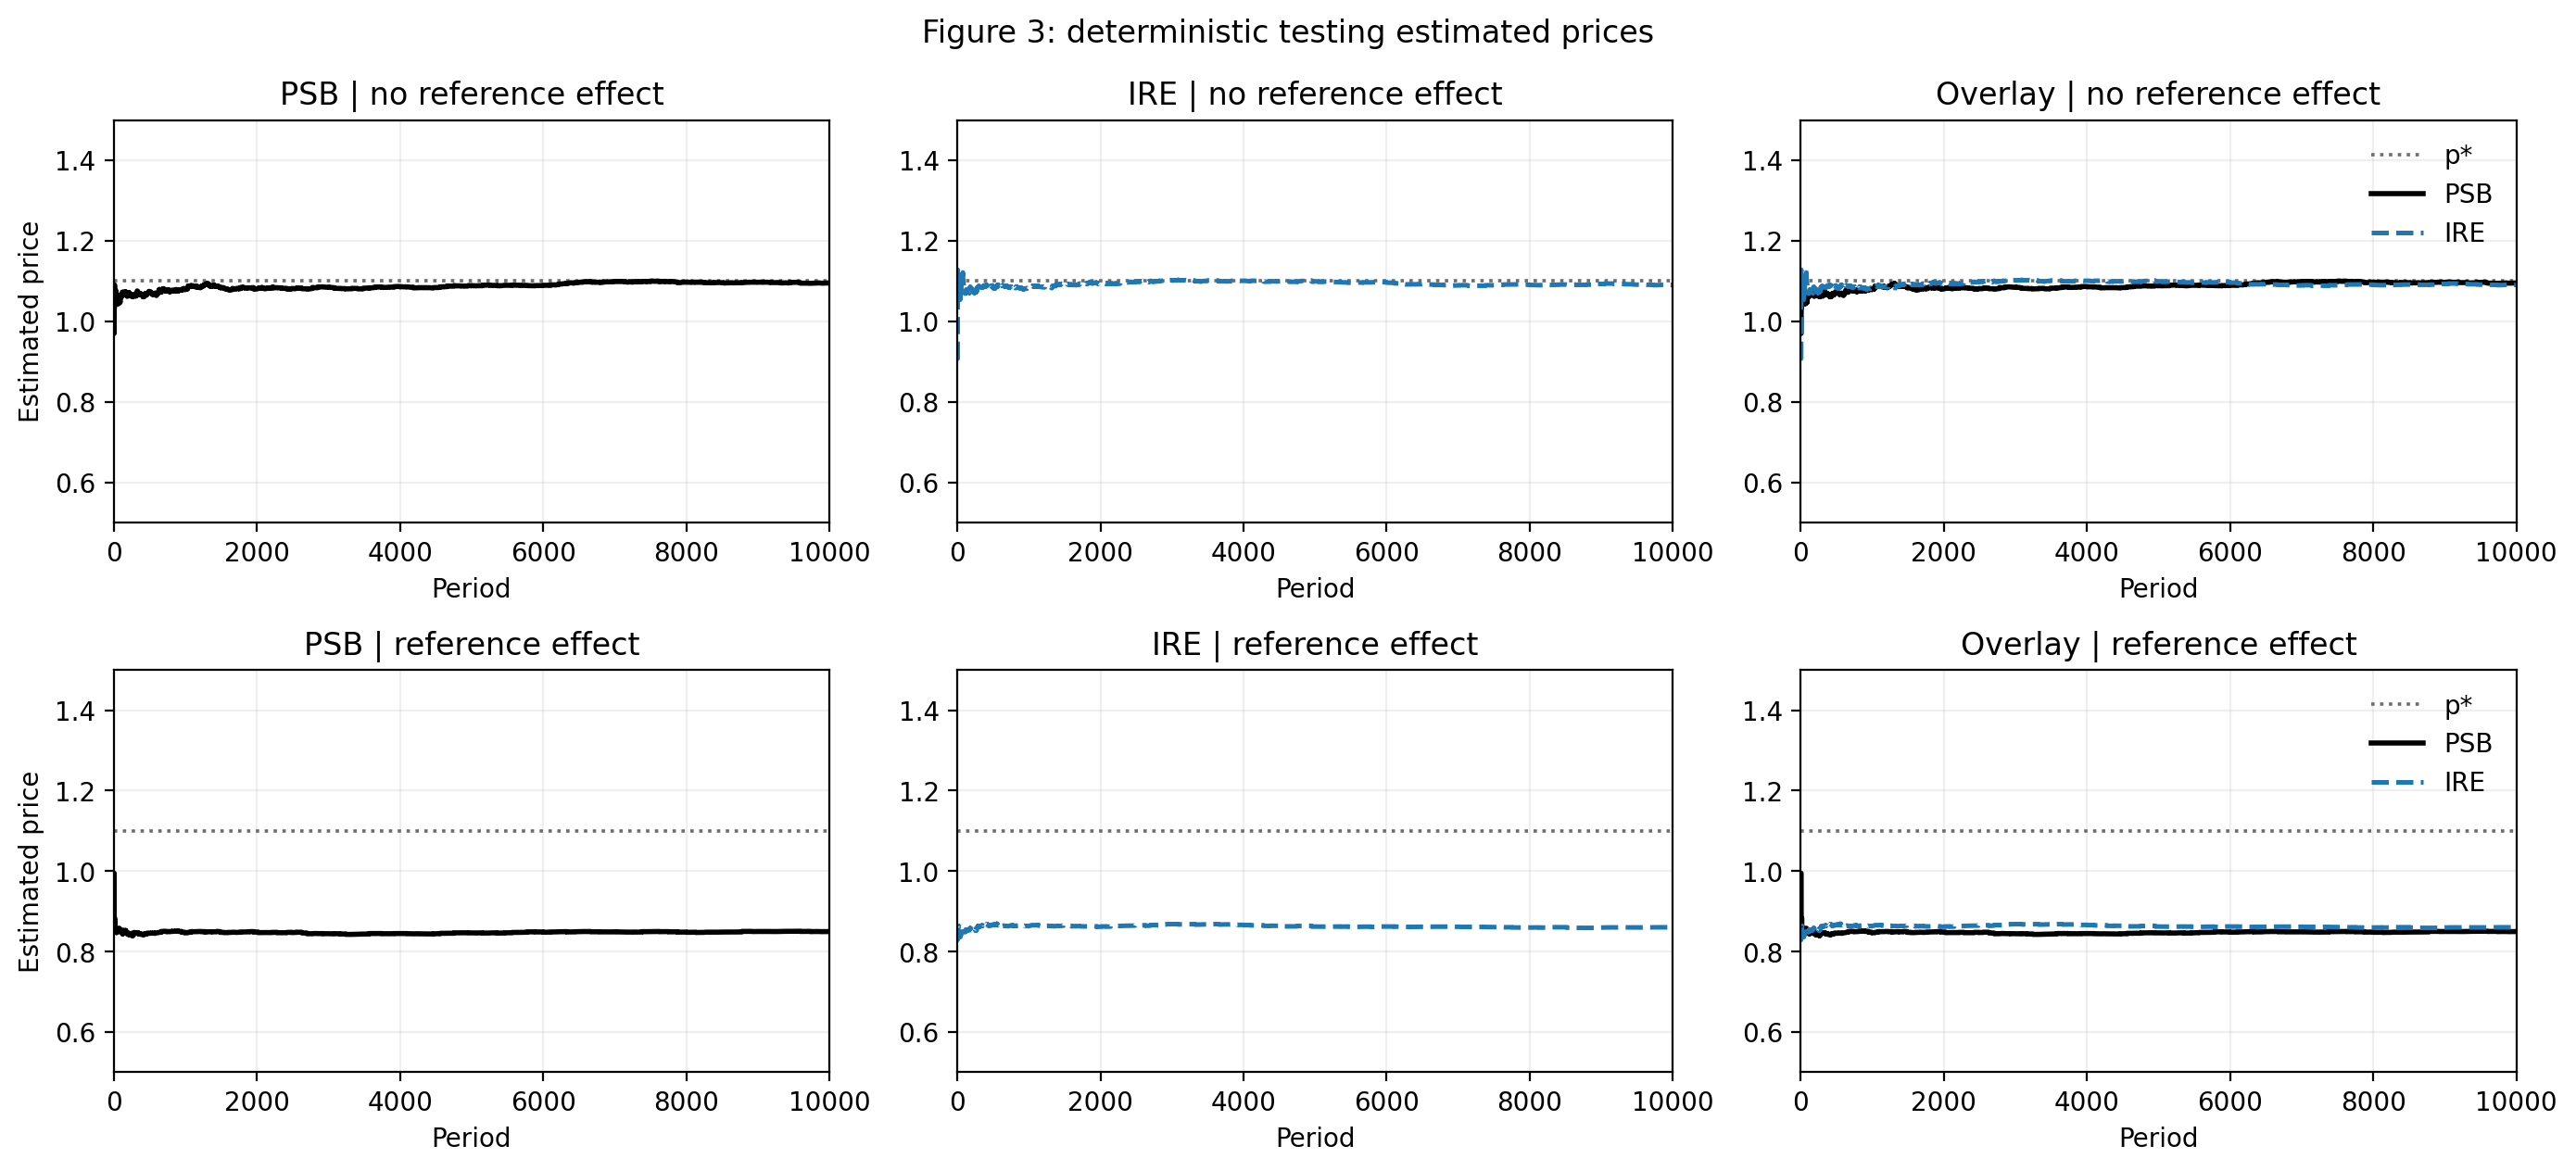
\includegraphics[width=0.96\textwidth]{figure3_comparison.png}
  \caption{Figure 3 comparison. Reference effects cause the deterministic-testing price estimate to stabilize below the benchmark.}
  \label{fig:figure3}
\end{figure*}

\subsection{Slow-Moving Pricing}
Figure~\ref{fig:figure4} focuses on the slow-moving policy in the reference-effect environment. The reference price and estimated price both move toward the neighborhood of $p^\star=1.1$. The final mean reference price is $1.097$ for PSB and $1.076$ for IRE. The final mean estimated price is $1.109$ for PSB and $1.088$ for IRE. These are small differences compared with the deterministic-testing bias in Figure~\ref{fig:figure3}.

\begin{figure*}[t]
  \centering
  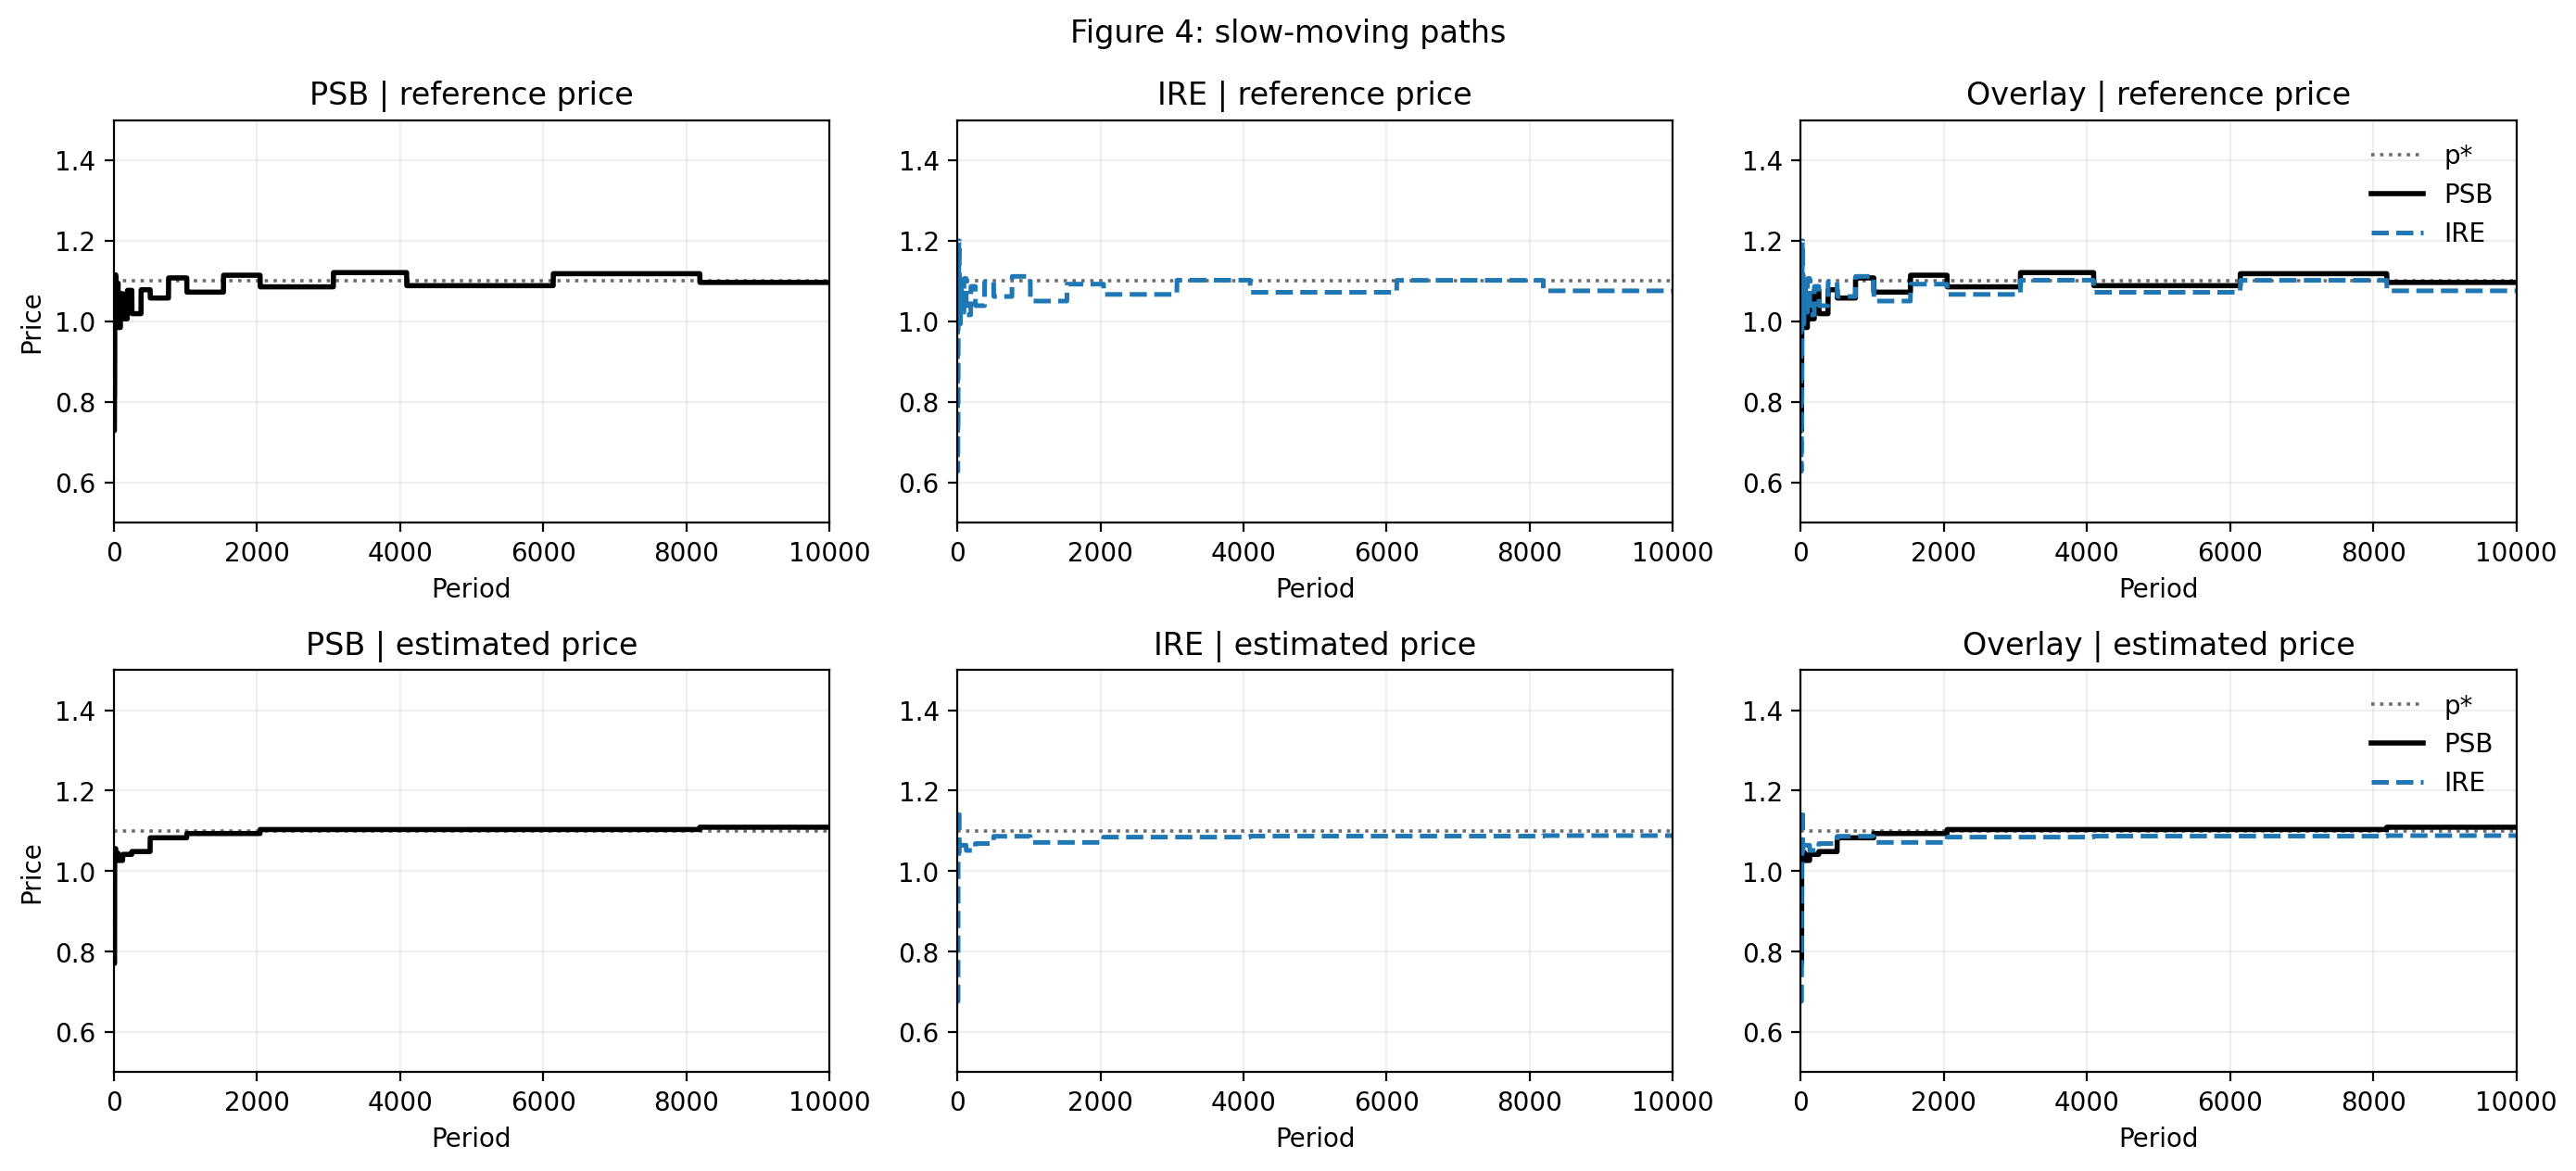
\includegraphics[width=0.96\textwidth]{figure4_comparison.png}
  \caption{Figure 4 comparison. Slow-moving pricing keeps the reference price and estimated price near the benchmark region.}
  \label{fig:figure4}
\end{figure*}

Figure~\ref{fig:figure5} shows regret under slow-moving pricing. The final IRE regret is $11.86$ without reference effects and $12.33$ with reference effects. The corresponding PSB values are $7.61$ and $10.40$. The exact values differ, but both environments remain in the same low-regret range. Compared with Figure~\ref{fig:figure2}, the important result is the order-of-magnitude contrast: deterministic testing jumps from roughly $10$ to roughly $300$ when reference effects are introduced, while slow-moving pricing remains near the low range.

\begin{figure*}[t]
  \centering
  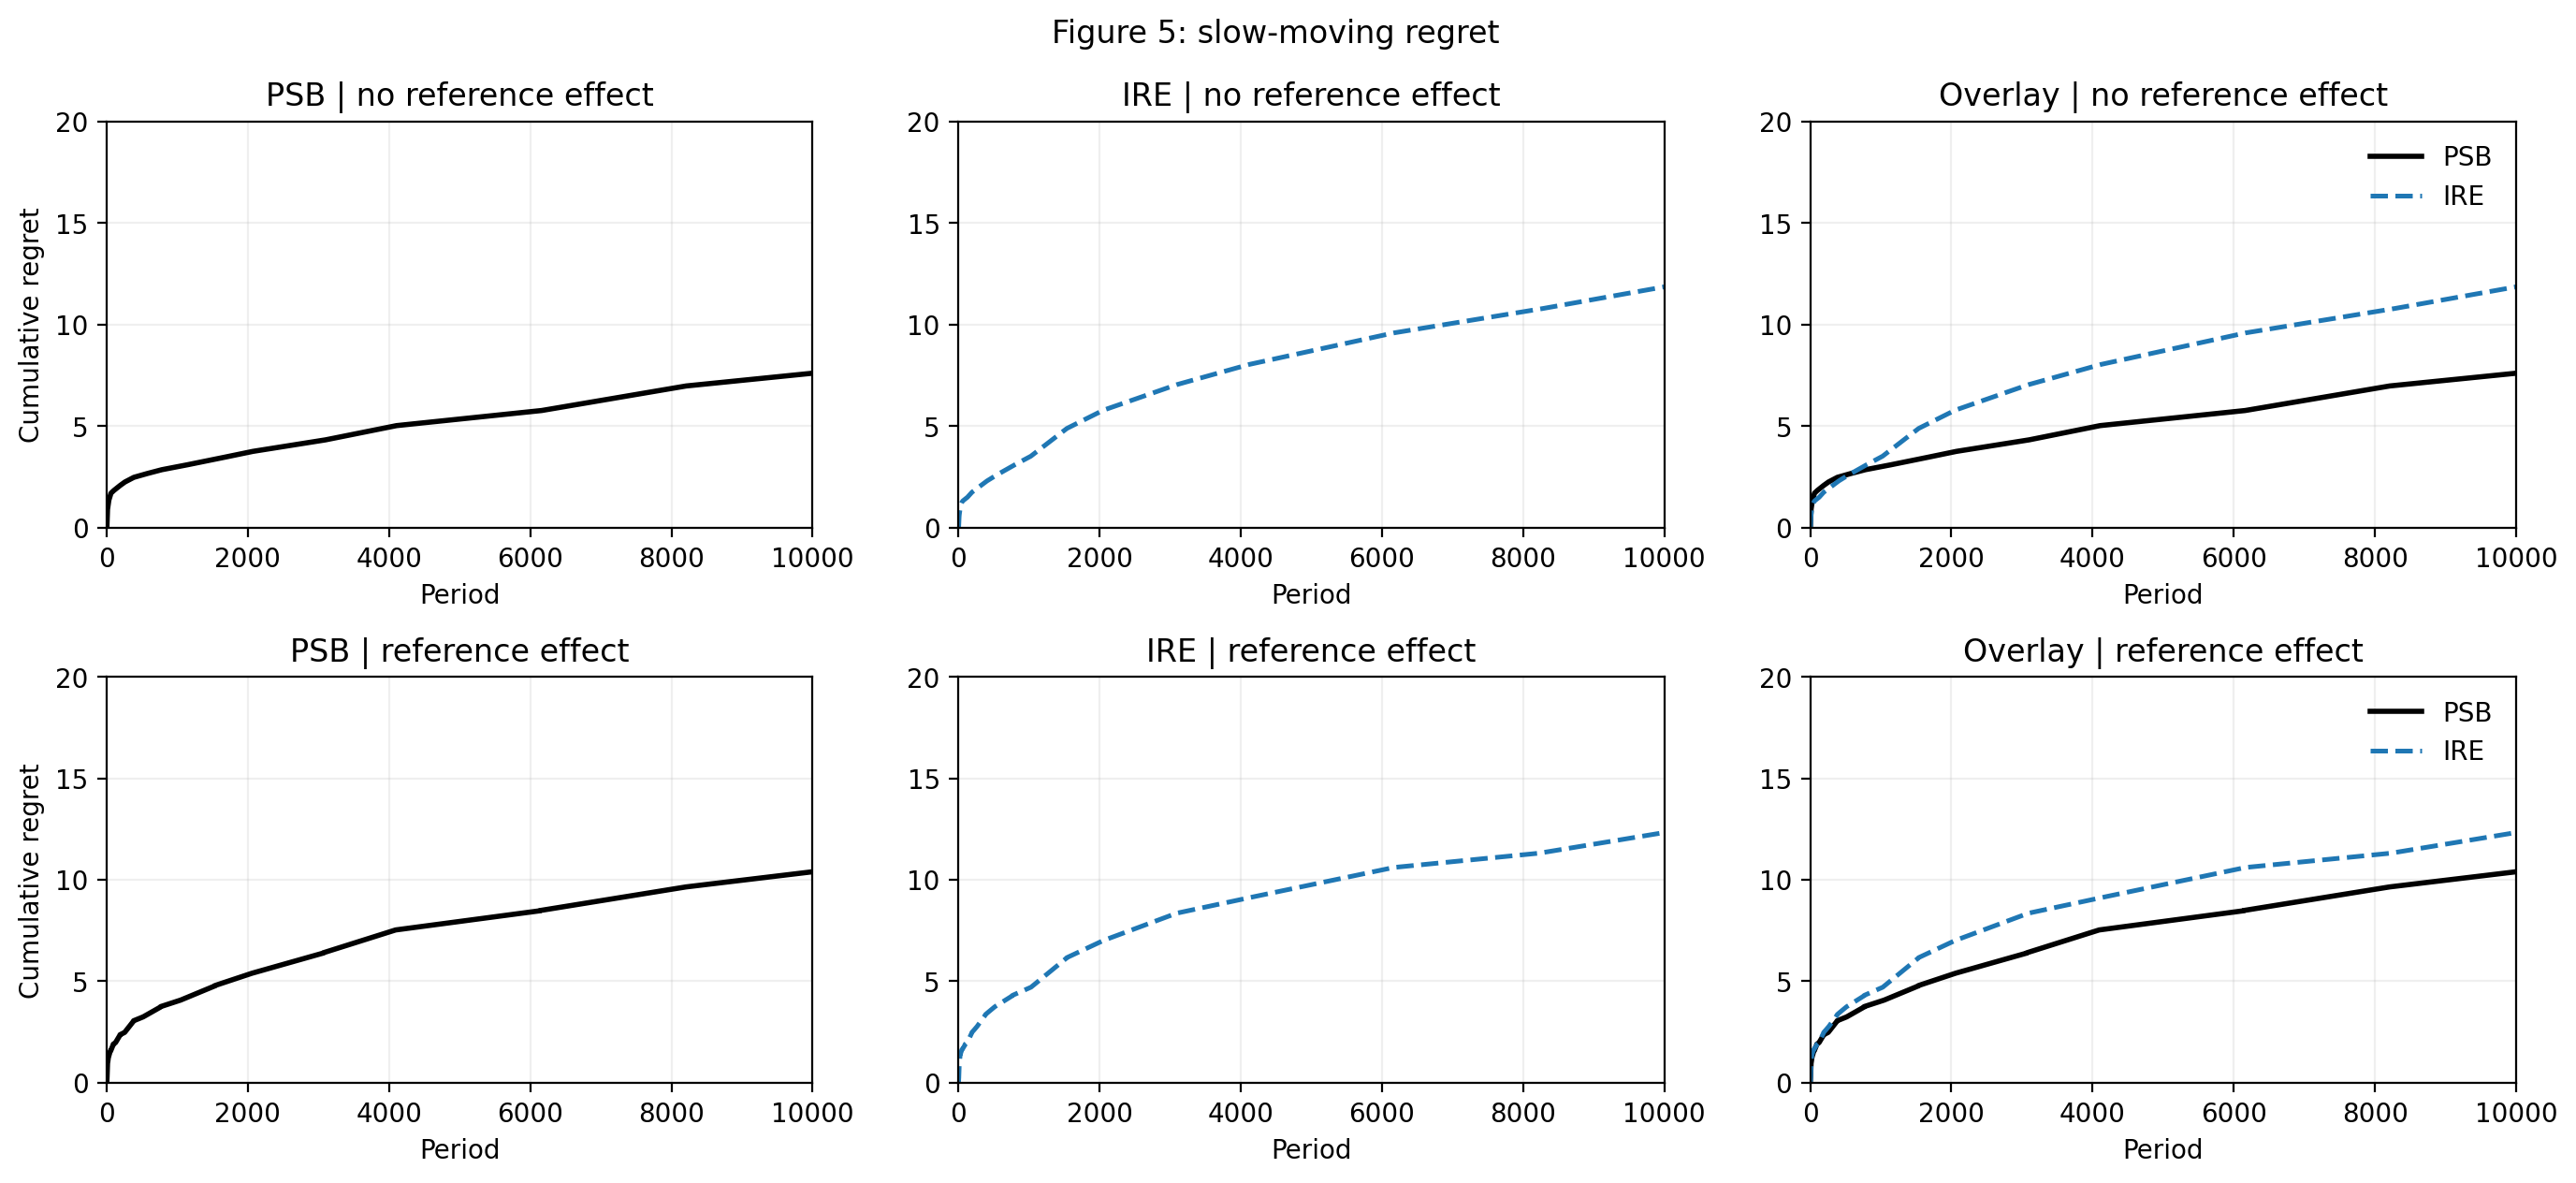
\includegraphics[width=0.96\textwidth]{figure5_comparison.png}
  \caption{Figure 5 comparison. Slow-moving pricing maintains low regret in both no-reference and reference-effect environments.}
  \label{fig:figure5}
\end{figure*}

\section{Mechanism-Level Analysis}
The replication results are best understood as a comparison between two kinds of exploration. Deterministic testing treats exploration as independent information collection. It posts two test prices at predetermined times, estimates a demand curve, and then exploits the estimate. This logic is valid when the demand shock is the only source of randomness and the demand curve depends only on current price. With reference effects, however, a test price is also a treatment that changes the reference state. The next demand observation is therefore affected by the current test.

Slow-moving pricing changes the information structure. By using long episodes, it allows the reference state to approach the current price region. By shrinking perturbations, it reduces the gap between exploration prices and the estimated optimum. This does not eliminate the reference effect, but it makes the state movement more predictable and less harmful for estimation. In this sense, slow-moving pricing converts a confounded learning problem into a more stable local learning problem.

This mechanism also explains why the comparison should focus on policy-level patterns, not on point-by-point equality. Different random streams can change individual paths and final values, especially with only ten simulation replications. The more important evidence is that the same structural contrast appears in both PSB and IRE: deterministic testing is robust in the no-reference environment and fragile in the reference-effect environment; slow-moving pricing is stable in both.

Figure~\ref{fig:policymechanism} visualizes this mechanism-level contrast. Deterministic testing produces large price jumps and then estimates demand from observations affected by the shifted reference state. Slow-moving pricing uses local perturbations and longer episodes to reduce this contamination.

\begin{figure*}[!t]
  \centering
  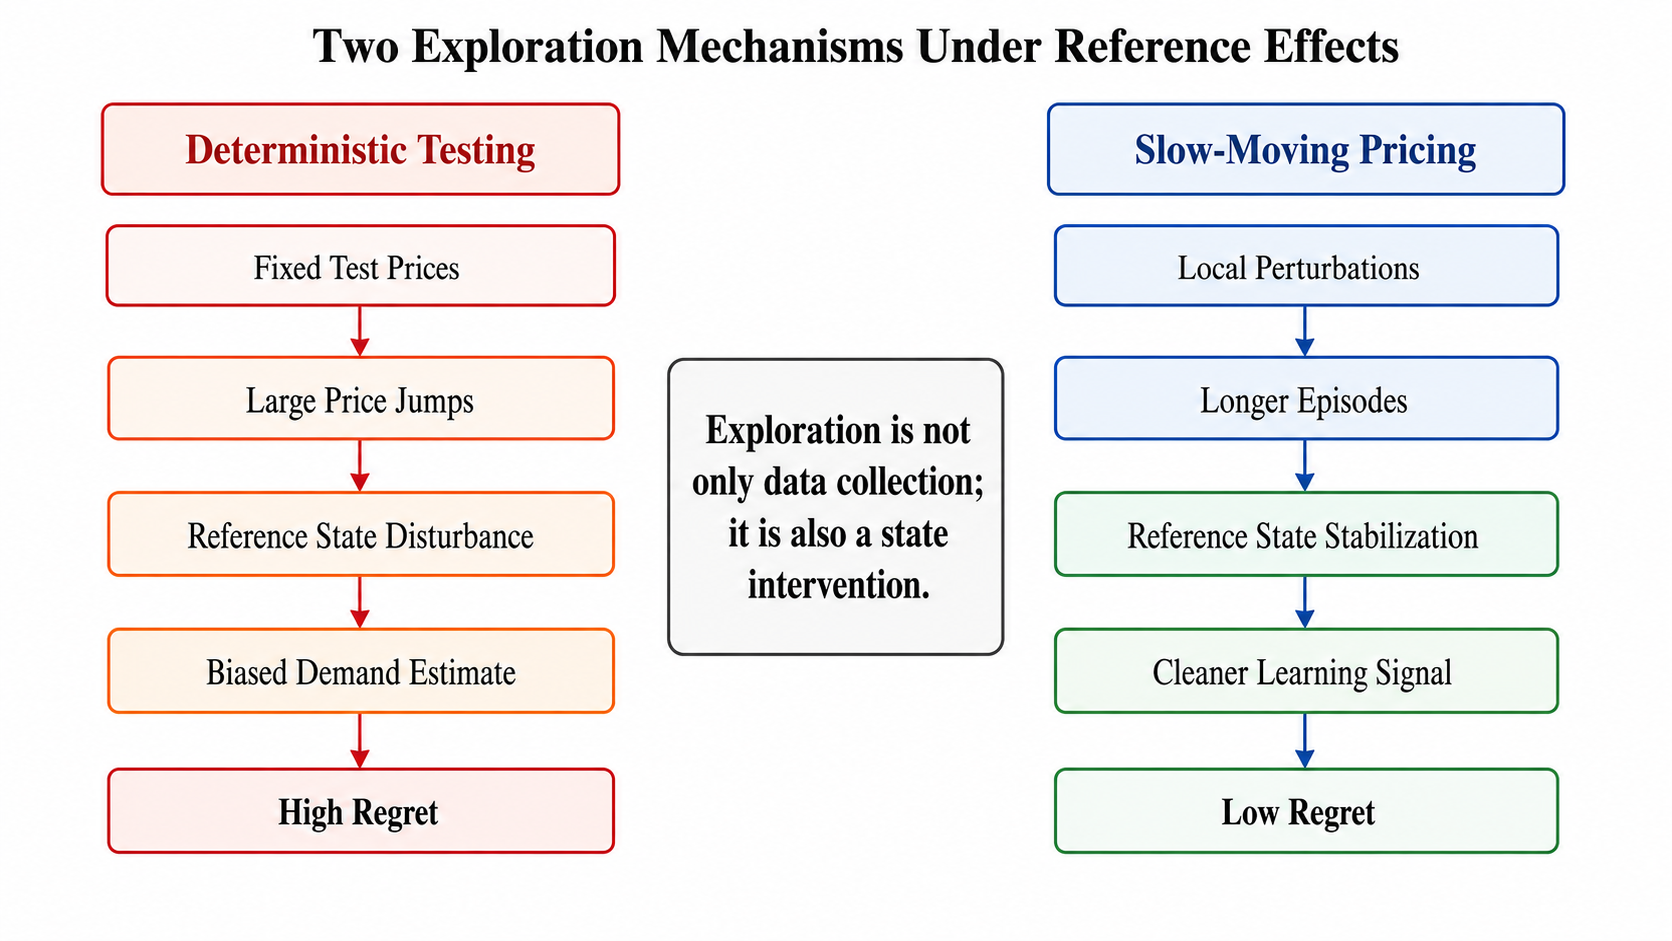
\includegraphics[width=0.92\textwidth]{exploration_mechanisms.png}
  \caption{Exploration mechanism comparison. Deterministic testing treats exploration as data collection, while slow-moving pricing treats exploration as a state-changing intervention.}
  \label{fig:policymechanism}
\end{figure*}

\begin{table*}[t]
\centering
\caption{Evidence map linking numerical outputs to the operations-research mechanism.}
\label{tab:evidence}
\resizebox{\textwidth}{!}{%
\begin{tabular}{llll}
\hline
Evidence & Main observation & Mechanism supported & Operational interpretation\\
\hline
Figure 2, no reference & Low deterministic-testing regret & Classical learning works when state is absent & Standard price testing is acceptable in a memoryless market\\
Figure 2, reference effect & Regret rises to about 300 & Forced tests move the reference state & Exploration can damage the future demand environment\\
Figure 3 & Estimated price stabilizes near 0.85 & State effect contaminates demand estimation & A biased plug-in price can look statistically stable\\
Figure 4 & Reference and estimated prices approach 1.1 & Slow episodes reduce state contamination & Gradual testing makes observations more reliable\\
Figure 5 & Slow-moving regret stays near the low range & Learning and state control are aligned & State-aware exploration prevents large long-run losses\\
RARC & Smaller perturbation is minimax-best & Tuning controls robustness under uncertainty & Calibration should account for behavioral-memory risk\\
\hline
\end{tabular}
}
\end{table*}

\section{Reproducibility Controls}
The implementation follows three reproducibility principles. First, the PSB data are converted before comparison and are not used directly by the IRE simulation. This makes the numerical comparison auditable: the converted arrays, CSV tables, and metadata files can be inspected separately from the simulation code. It also avoids mixing the source format with the experiment logic.

Second, realized demand and expected revenue are separated. Realized demand includes the random shock and is used for estimator updates. Regret is computed from expected revenue, which is consistent with the theoretical definition of performance. This distinction is important because otherwise the regret curve would mix policy loss with realized demand noise, making the result harder to interpret.

Third, all random streams in the IRE are deterministic. The project does not attempt to match the PSB path by path, but deterministic seeds make the IRE results exactly reproducible from the command line. This is useful for grading and for later extensions: if a new policy changes the result, the change can be attributed to the policy rather than to a different random draw.

The code is organized by model component. The demand function, reference-price update, least-squares estimator, pricing policies, regret metrics, data conversion, and plotting are separated into modules. This design is not only a software convenience. It mirrors the mathematical structure of the paper: demand, state evolution, learning, control, and evaluation are different objects. Separating them reduces the risk of using realized demand where expected revenue is required, or using a state update inside a policy where it should only be part of the environment.

The validation strategy has two levels. Unit tests check formula-level behavior, including the two sides of the reference-effect demand function, exponential reference updating, static optimal pricing, least-squares recovery, and expected-revenue regret. CLI smoke tests then run a short horizon to verify that directories, arrays, CSV files, and figures are generated consistently. The full run uses the default horizon and simulation count to generate the results used in this report.

\section{Novel Extension: Reference-Aware Robust Calibration}
\subsection{Motivation}
The main replication uses the slow-moving policy with $c_0=0.10$ and perturbation decay exponent $0.25$. These values reproduce the published numerical design, but applied settings rarely know the exact reference-memory parameter or the exact loss-side reference-effect coefficient. A retailer may know that consumers are loss averse, but not whether the reference price updates very quickly or moderately slowly. It may also know that losses matter more than gains, but not the precise value of $\eta^-$.

To address this issue, this project adds Reference-Aware Robust Calibration (RARC). RARC is not a new proof of optimality. It is a numerical operations-research extension that asks how the slow-moving perturbation parameters should be chosen when the reference process is uncertain. It converts the replication from a single-parameter experiment into a small robust-design problem.

\subsection{Experimental Design}
The uncertainty set varies the reference-memory parameter and the loss-side reference effect:
\begin{equation}
\zeta \in \{0.02,0.10,0.40\},\quad
\eta^- \in \{0.15,0.30,0.45\},
\end{equation}
with $\eta^+=0.10$. The candidate policy set varies the initial perturbation scale and the perturbation decay exponent:
\begin{equation}
c_0 \in \{0.05,0.10,0.15\},\quad
\gamma \in \{0.20,0.25,0.30\},
\end{equation}
where $\delta_i=c_0 2^{-\gamma i}$ in the generalized slow-moving schedule. The candidate $(c_0,\gamma)=(0.10,0.25)$ is the default replication setting. RARC evaluates each candidate on all nine environments and records average final regret, worst-case final regret, and average path regret.

Figure~\ref{fig:rarcworkflow} shows the RARC workflow. The extension combines a behavioral uncertainty set with a schedule-candidate grid, evaluates each policy-environment pair, and selects default, mean-best, and minimax-best candidates using robust regret metrics.

\begin{figure*}[!t]
  \centering
  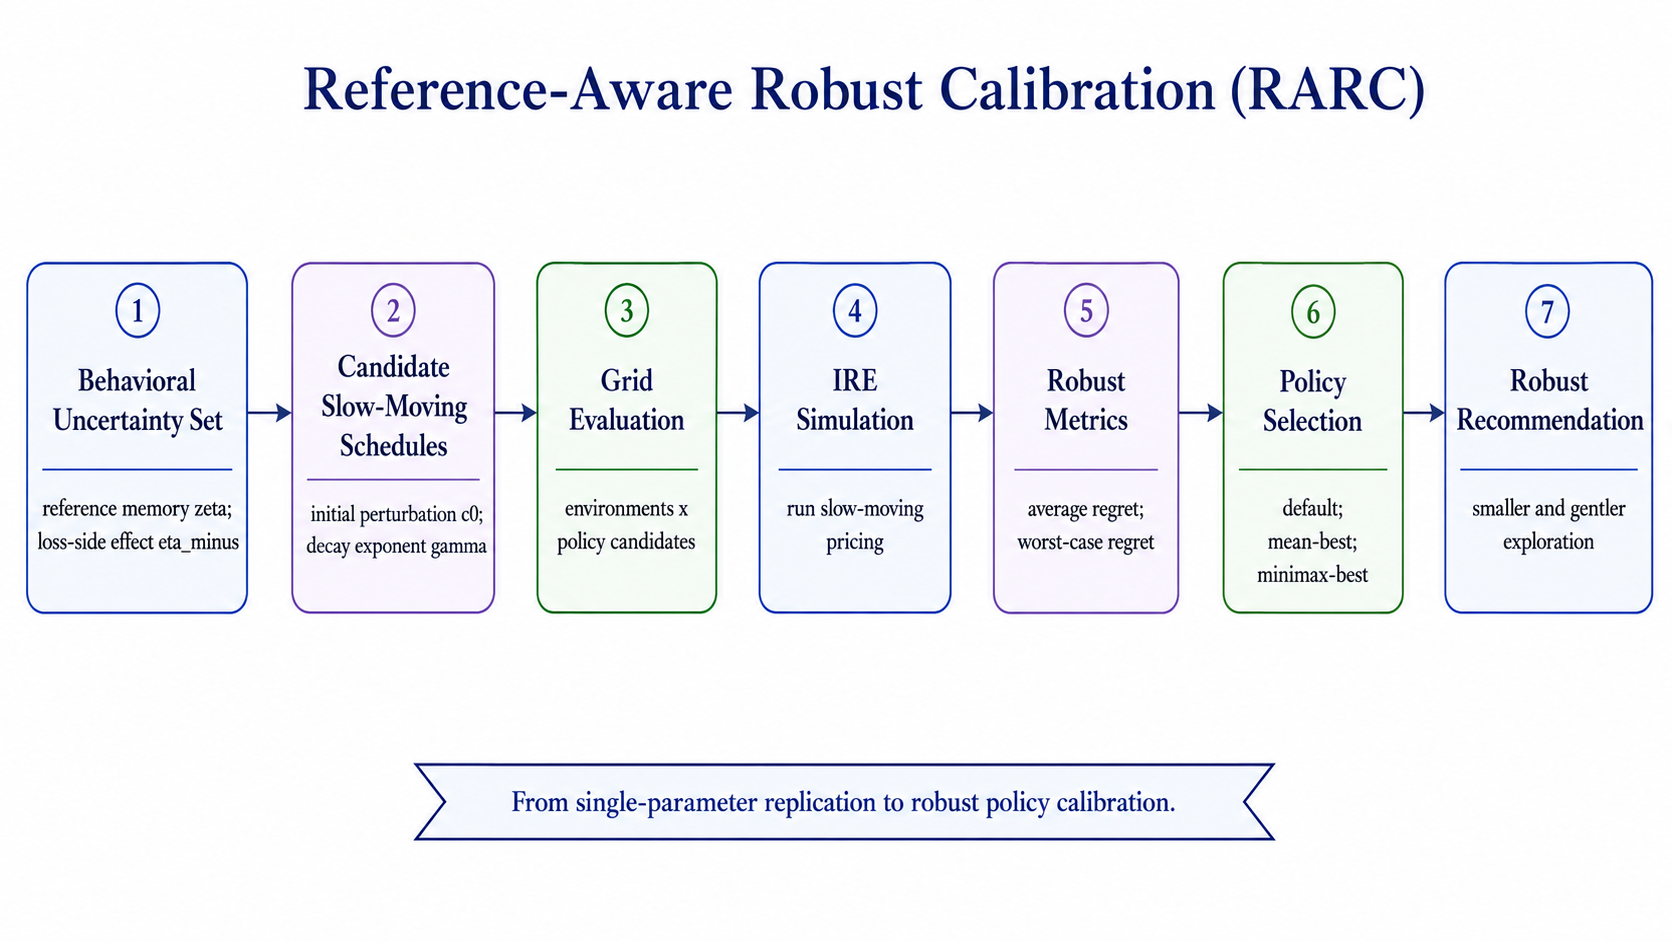
\includegraphics[width=0.92\textwidth]{rarc.png}
  \caption{RARC workflow. The extension turns slow-moving schedule selection into a robust calibration problem over behavioral uncertainty.}
  \label{fig:rarcworkflow}
\end{figure*}

\subsection{RARC Results}
Table~\ref{tab:rarc} shows the main RARC summary. The default candidate remains strong: its average final regret is $13.09$ and its worst-case final regret is $14.39$. However, the best candidate in both average and minimax terms is $(c_0,\gamma)=(0.05,0.20)$, with average final regret $10.62$ and worst-case final regret $13.32$. The largest tested initial perturbation, $c_0=0.15$, performs worse, especially when paired with faster decay in hard environments.

\begin{table*}[t]
\centering
\caption{RARC candidate summary across nine uncertainty-set environments.}
\label{tab:rarc}
\begin{tabular}{lrrrrl}
\hline
Candidate & $c_0$ & Decay exponent & Average final regret & Worst-case final regret & Role\\
\hline
c0\_0\_05\_decay\_0\_20 & 0.05 & 0.20 & 10.62 & 13.32 & mean-best; minimax-best\\
c0\_0\_05\_decay\_0\_25 & 0.05 & 0.25 & 10.70 & 13.78 & candidate\\
c0\_0\_05\_decay\_0\_30 & 0.05 & 0.30 & 10.82 & 14.19 & candidate\\
c0\_0\_10\_decay\_0\_25 & 0.10 & 0.25 & 13.09 & 14.39 & default\\
c0\_0\_15\_decay\_0\_30 & 0.15 & 0.30 & 17.12 & 24.35 & high-risk candidate\\
\hline
\end{tabular}
\end{table*}

Table~\ref{tab:environment} reports the environment-level stress pattern. The easiest environments are those with low memory and low loss-side reference effect. The hardest environment is $\zeta=0.40$ and $\eta^-=0.45$, where the average candidate regret reaches $17.06$ and the worst tested candidate reaches $24.35$. This is consistent with the model: a more persistent reference state and a stronger loss penalty make state contamination more expensive.

\begin{table*}[t]
\centering
\caption{RARC environment summary across all candidate schedules.}
\label{tab:environment}
\begin{tabular}{rrrrr}
\hline
$\zeta$ & $\eta^-$ & Average final regret & Best final regret & Worst final regret\\
\hline
0.02 & 0.15 & 12.18 & 9.44 & 15.44\\
0.02 & 0.30 & 12.65 & 9.76 & 16.73\\
0.02 & 0.45 & 13.71 & 10.63 & 17.22\\
0.10 & 0.15 & 12.34 & 9.51 & 15.64\\
0.10 & 0.30 & 12.96 & 9.90 & 17.04\\
0.10 & 0.45 & 13.99 & 10.96 & 17.72\\
0.40 & 0.15 & 13.41 & 10.37 & 16.79\\
0.40 & 0.30 & 15.14 & 11.40 & 20.80\\
0.40 & 0.45 & 17.06 & 13.32 & 24.35\\
\hline
\end{tabular}
\end{table*}

Figure~\ref{fig:rarc} visualizes the same conclusion. The heatmaps show that smaller perturbations dominate larger perturbations over this uncertainty set. The frontier panel shows that the mean-best and minimax-best selections coincide. This indicates that the chosen robust candidate is not only protecting against one extreme environment; it also improves average performance across the grid.

\begin{figure*}[t]
  \centering
  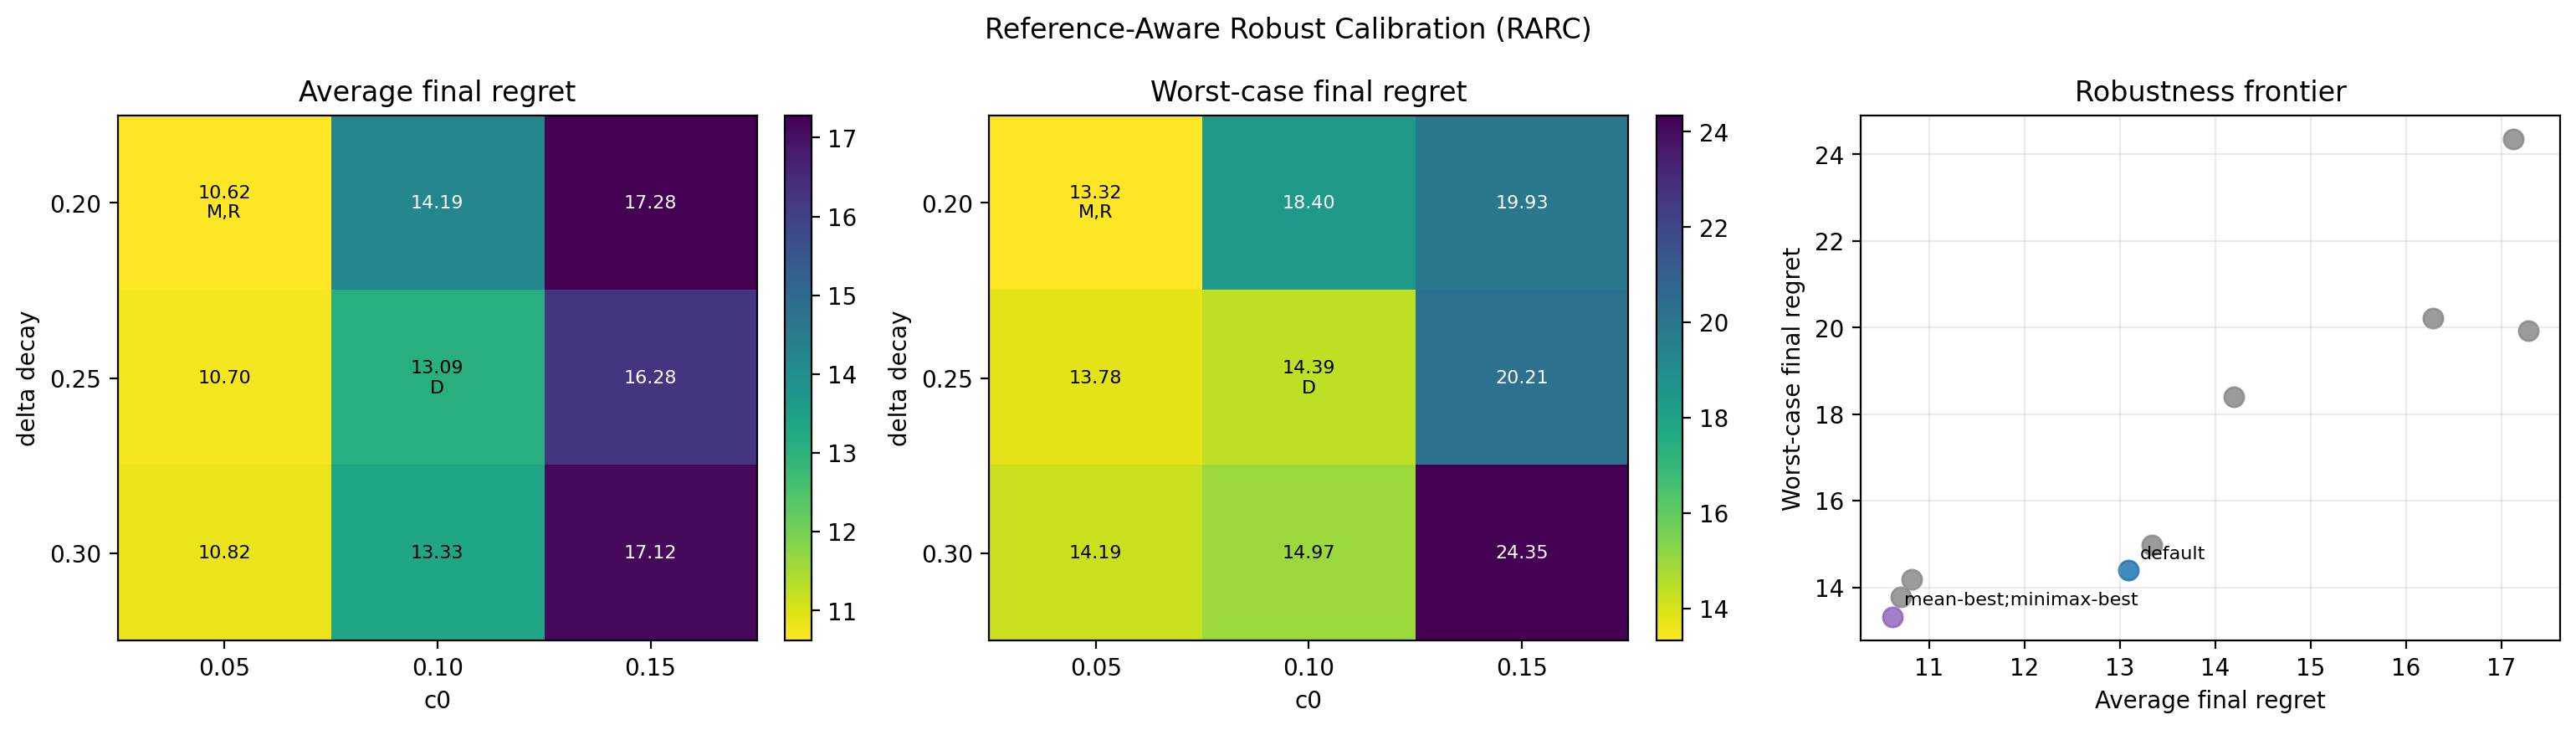
\includegraphics[width=0.96\textwidth]{robust_calibration.png}
  \caption{RARC extension. Heatmaps compare average and worst-case final regret; the frontier panel compares average and worst-case performance.}
  \label{fig:rarc}
\end{figure*}

The operations-research interpretation is practical. The slow-moving idea is structurally correct, but its tuning matters. If perturbations are too large, the policy creates unnecessary revenue loss and larger reference-state movements. If perturbations decay too quickly after a large initial scale, the policy can still carry early-state damage into later periods. In this experiment, a smaller initial perturbation with slower decay is more robust. This is consistent with the paper's mechanism: exploration should be local enough to control reference-state contamination.

\subsection{What RARC Adds}
RARC adds a design layer that is not visible in the original Figure 2--5 replication. The replication asks whether the slow-moving structure works under one calibrated environment. RARC asks whether the schedule is stable when the behavioral environment changes. This is closer to a practical pricing problem, where the firm may not know the exact memory length or the exact magnitude of loss aversion before running experiments.

The RARC result also clarifies the role of exploration size. Large perturbations are not automatically better because they generate more variation. In a reference-price model, variation has two prices: it creates statistical information, and it changes the customer reference state. The best candidate in the tested grid uses a smaller initial perturbation, suggesting that the marginal value of extra price dispersion is lower than the state-control cost in these environments.

Finally, RARC provides a natural starting point for future algorithm design. A fully adaptive policy could begin with a conservative schedule and update its perturbation scale as it learns about both demand and reference-memory strength. The present RARC experiment does not implement that adaptive loop, but it identifies the relevant design variables and shows that they matter numerically.

\section{Operations Research Discussion}
\subsection{Robust Optimization Perspective}
The RARC extension can be interpreted as a small robust-optimization problem. The decision variables are the schedule parameters $c_0$ and $\gamma$. The uncertainty set contains plausible values of the behavioral parameters $\zeta$ and $\eta^-$. The objective is not only to perform well in an average environment, but also to avoid poor outcomes in the hardest environment. This is a natural fit for operations research, where decision makers often choose policies before all model parameters are known.

The minimax view changes how the slow-moving policy is evaluated. A schedule that is attractive for a single calibrated environment may be less attractive if it has high regret under a slightly more persistent reference state. Conversely, a conservative schedule can be valuable if it limits downside risk with only a small average-cost penalty. In the tested grid, the same candidate minimizes both average and worst-case final regret, which makes the recommendation operationally simple.

\subsection{Online Learning Perspective}
The paper illustrates an important lesson for online learning. Data generated by a policy are not always passive observations. In many operational systems, actions change future states and therefore change the distribution of later observations. This creates feedback between learning and control. Deterministic testing fails because it ignores that feedback; slow-moving pricing succeeds because it controls the feedback channel.

This point connects the paper to broader learning-and-control problems such as inventory experiments, platform ranking, and promotion planning. In each case, an experiment can change customer behavior, inventory position, or future demand composition. A good policy must be evaluated by long-run system response, not only by short-run estimation accuracy. The regret framework is useful because it captures this cumulative effect.

\subsection{Managerial Perspective}
For a manager, the main lesson is that price experimentation should be gradual when customers remember prices. A sharp discount may generate useful data and short-run sales, but it may also reset reference prices downward. A sudden price increase may reveal demand elasticity, but it may also create loss perceptions. The slow-moving policy suggests a disciplined alternative: use local tests around a current estimate, let the market state settle, and update only after enough observations are collected.

RARC adds a practical rule for uncertain markets. If the firm is unsure about consumer memory and loss aversion, starting with a smaller perturbation can be safer than using aggressive tests. This does not mean that exploration should disappear. It means that exploration intensity should be chosen with both statistical information and behavioral-state cost in mind.

\section{Strengths, Limitations, and Future Extensions}
\subsection{Strengths}
The main strength of the method is conceptual clarity. It identifies why a standard learning policy fails: the policy ignores the fact that price experiments alter future demand states. The slow-moving policy is also interpretable. It uses episodes, two-sided perturbations, and ordinary least squares rather than a complex black-box optimizer. This makes it easier to explain as a managerial testing protocol.

The numerical evidence is strong because the two policies are compared under the same model parameters and the same performance metric. Figure~\ref{fig:figure2} and Figure~\ref{fig:figure5} form a clean contrast. Ignoring reference effects produces a large regret increase, while controlling the reference state prevents that increase. The RARC extension adds another strength: it turns the policy schedule into a tunable robust-design object.

\subsection{Limitations}
The study also has important limitations. First, the demand model is synthetic and linear. Real demand may be nonlinear, censored by inventory, affected by competitors, or shaped by covariates such as seasonality and customer segment. Second, the number of simulation paths is small, so exact final values should not be overinterpreted. Third, the slow-moving policy is designed for the loss-averse time-varying reference-price setting. Other behavioral regimes, such as gain-seeking customers, can imply different optimal price paths. Fourth, the RARC extension is numerical. It suggests a robust tuning direction, but it does not prove a new regret bound for the selected candidate.

\subsection{Possible Extensions}
Theoretical extensions could weaken the assumptions on the reference-price process. For example, future work could study heterogeneous memory rates, random jumps in reference prices, or partially observed reference-state distributions. The key question is whether $O(\sqrt{T})$ regret can be preserved when the state process is more persistent or less predictable.

Algorithmic extensions could combine slow-moving pricing with confidence intervals or Bayesian learning. Instead of using a fixed perturbation decay rule, the policy could adapt $c_0$ and $\gamma$ to estimation uncertainty and state-contamination risk. RARC is a first step in this direction because it treats schedule choice as a robust calibration problem.

Application extensions include promotion calendars, subscription renewal pricing, and platform price experiments. A practical firm should not evaluate a pricing experiment only by immediate sales lift. It should also measure how the experiment changes customer expectations. That requires combining pricing analytics with behavioral indicators such as search behavior, repeat purchase patterns, and responses to repeated discounts.

\begin{table}[H]
\centering
\footnotesize
\setlength{\tabcolsep}{1pt}
\caption{Future extension roadmap.}
\label{tab:roadmap}
\begin{tabular}{p{0.14\columnwidth}p{0.31\columnwidth}p{0.25\columnwidth}p{0.22\columnwidth}}
\hline
Direction & Research question & Possible method & Expected contribution\\
\hline
Theory & Can regret guarantees survive richer reference processes? & General state-deviation bounds & Broader conditions for $O(\sqrt{T})$ behavior\\
Theory & How does consumer heterogeneity change learning? & Latent-state or mixture models & Segment-level reference-price control\\
Alg. & Can perturbations adapt online? & Confidence intervals or Bayesian updates & State-aware adaptive exploration\\
Alg. & Can RARC be made sequential? & Minimax or distributionally robust tuning & Robust schedules without fixed grids\\
App. & How should promotions be scheduled? & Calendar constraints with reference states & Lower long-run promotion damage\\
App. & How can firms measure reference effects? & Linking transactions with behavioral signals & Field-ready reference-state estimation\\
\hline
\end{tabular}
\end{table}

\section{Conclusion}
This project reproduces and extends the main numerical lesson of den Boer and Keskin \cite{denBoerKeskin2022}. Dynamic pricing with reference effects differs fundamentally from ordinary demand learning because price choices create the state that affects future observations. Deterministic testing performs well when reference effects are absent, but it becomes misspecified when reference effects are present. Slow-moving pricing succeeds because it designs exploration and reference-state control together.

The RARC extension adds a practical calibration message. Within the tested uncertainty set, the default slow-moving schedule is robust, but a smaller initial perturbation and slower decay achieve lower average and worst-case final regret. This supports the broader operations-research principle behind the paper: in dynamic systems with endogenous behavioral states, the best learning algorithms are not just statistically efficient; they are also careful about how their actions reshape the system being learned.

\bibliographystyle{IEEEtran}
\bibliography{../bib/references}

\end{document}
